\documentclass[10pt,a4paper]{article}
\usepackage{amsmath}

%%%%%%%%%%%%%%%%%%%%%%%%%%%
% MODIFY:

\newcommand{\authorA}{ALEX PASQUALI (03754113)}
\newcommand{\authorB}{NICOLA GUGOLE (03753996)}
\newcommand{\groupNumber}{A} % - YOUR GROUP
\newcommand{\exerciseNumber}{3} % - THE NUMBER OF THE EXERCISE
\newcommand{\sourceCodeLink}{\url{https://github.com/AlexPasqua/MLCMS-exercises}}

\newcommand{\workPerAuthor}{
\authorA&Task 1&50\%\\
      &Task 2&50\%\\
      &Task 3&50\%\\
      &Task 4&50\%\\
      &Task 5&50\%\\
      \hline
\authorB&Task 1&50\%\\
      &Task 2&50\%\\
      &Task 3&50\%\\
      &Task 4&50\%\\
      &Task 5&50\%\\
}

%%%%%%%%%%%%%%%%%%%%%%%%%%%

%%
% imports for the exercise sheets
%

\usepackage[utf8]{inputenc}
\usepackage{amsmath}
\usepackage{amsfonts}
\usepackage{amssymb}

\usepackage[yyyymmdd]{datetime}
\renewcommand{\dateseparator}{--}

\usepackage[left=2cm,right=2cm,top=3cm,bottom=3cm]{geometry}

\usepackage{hyperref}

\usepackage{amsthm}
\newtheorem{lem}{Lemma}
\newtheorem{thm}{Theorem}
\newtheorem{cor}{Corollary}
\newtheorem{rem}{Remark}
\newtheorem{definition}{Definition}
\newtheorem{ter}{Terminology}

\usepackage{graphicx}

\newcommand{\M}{\mathcal{M}}
\newcommand{\N}{\mathcal{N}}
\newcommand{\K}{\mathcal{K}}
\newcommand{\SPDk}{\mathbb{P}^k}
\newcommand{\vol}{\text{vol}}

\newcommand{\Figref}[1]{Figure~\ref{#1}}
\newcommand{\figref}[1]{figure~\ref{#1}}
\newcommand{\Eqnref}[1]{Equation~(\eqref{#1})}
\newcommand{\eqnref}[1]{equation~(\eqref{#1})}

\usepackage{float}
\usepackage{tabularx}

\usepackage{fancyhdr}
\pagestyle{fancy}

\usepackage{totcount}
\newtotcounter{taskCounter}
\newtotcounter{pointCounter}
\newenvironment{task}[1]{\noindent\stepcounter{taskCounter}\textbf{Report on task #1}\smallbreak\hrule\smallbreak}{\smallbreak\hrule\bigbreak}


\title{Report for exercise \exerciseNumber~from group~\groupNumber}

\makeatletter
\let\thetitle\@title
\let\theauthor\@author
\let\thedate\@date
\makeatother

\providecommand{\versiondate}{\today}

\lhead{Exercise sheet \exerciseNumber}
\chead{Master Praktikum: Modelling and Simulation of Crowds WS2019/20}
\rhead{TUM}
\lfoot{Report of Group \groupNumber}
\cfoot{\thepage}
\rfoot{Last compiled: \versiondate}
\renewcommand{\headrulewidth}{0.4pt}
\renewcommand{\footrulewidth}{0.4pt}

\newcommand{\frontpage}{
\begin{center}
\textbf{\thetitle}\\~\\
\end{center}
\begin{table}[H]
\begin{tabular}{ll}
Tasks addressed:&\total{taskCounter}\\
Authors:&\authorA\\
&\authorB\\
&\authorC\\
Last compiled:&\versiondate\\
Source code:&\sourceCodeLink
\end{tabular}
\end{table}
\vfill
The work on tasks was divided in the following way:
\begin{table}[H]
\begin{tabularx}{\textwidth}{X|p{2cm}|p{2cm}}
\workPerAuthor
\end{tabularx}
\end{table}
\newpage
}

\begin{document}

\frontpage

\begin{task}{1, Vector fields, orbits, and visualization}
This tasks consists of displaying the phase portraits displayed in figure 2.5 of \cite{kuznetsov}.
In particular they are a \textit{node} and a \textit{focus} phase portraits, both \textit{stable} and \textit{unstable}, plus an \textit{unstable saddle} phase portrait.\\
The linear dynamical system in object has a state space $X=\mathbb{R}^2$, $I=\mathbb{R}$ and parameter $\alpha\in\mathbb{R}$.
Its flow is defined as follows:
\begin{equation}\label{eq:sys-task1}
    \frac{\partial\phi_{\alpha}(t,x)}{\partial t}\Bigr|_{t=0}=A_{\alpha}x
\end{equation}
where $x\inX$, $t\in I$ and $A$ is a 2x2 real matrix parametrized by $\alpha$.
Specifically, we obtained these portraits with the following configurations
(where $\lambda_1$ and $\lambda_2$ indicate the 2 eigenvalues of $A$):
\begin{itemize}
    \item \textbf{Unstable focus:} $\alpha=0.1,\ A=
    \begin{bmatrix}
    \alpha & \alpha \\
    -\frac{1}{4} & 0
    \end{bmatrix},\
    \lambda_1 = 0.05+0.15i,\ \lambda_2 = 0.05-0.15i$
    
    \item \textbf{Unstable saddle:} $\alpha=-0.2,\ A=
    \begin{bmatrix}
    -\alpha & \alpha \\
    -\frac{1}{4} & 0
    \end{bmatrix},\
    \lambda_1 = 0.345,\ \lambda_2 = -0.145$
    
    \item \textbf{Unstable node:} $\alpha=2,\ A=
    \begin{bmatrix}
    \alpha & \alpha \\
    -\frac{1}{4} & 0
    \end{bmatrix},\
    \lambda_1 = 1.707,\ \lambda_2 = 0.293$
    
    \item \textbf{Stable node:} $\alpha=-0.25,\ A=
    \begin{bmatrix}
    \alpha & 0 \\
    0 & -1
    \end{bmatrix},\
    \lambda_1 = -0.25,\ \lambda_2 = -1$
    
    \item \textbf{Stable focus:} $\alpha=0.1,\ A=
    \begin{bmatrix}
    -\alpha & \alpha \\
    -\frac{1}{4} & 0
    \end{bmatrix},\
    \lambda_1 = -0.05+0.15i,\ \lambda_2 = -0.05-0.15i$
\end{itemize}
These systems are of course \textbf{not} topologically equivalent because their phase portraits (\hyperref[fig:task1-phase-portraits]{Figure \ref{fig:task1-phase-portraits}}) show qualitatively distinct behaviors around their fixed point.
In particular, some of them are stable (Figure \ref{fig:task1-phase-portraits}(d) and \ref{fig:task1-phase-portraits}(e)) and some unstable (Figure \ref{fig:task1-phase-portraits}(a), \ref{fig:task1-phase-portraits}(b) and \ref{fig:task1-phase-portraits}(c)).
Moreover, Figure \ref{fig:task1-phase-portraits}(a)-(e) represent focuses,
Figure  \ref{fig:task1-phase-portraits}(b) represents a saddle and Figure \ref{fig:task1-phase-portraits}(c)-(d) represent nodes.

\begin{figure}[H]
    \centering
    \subfloat[a]{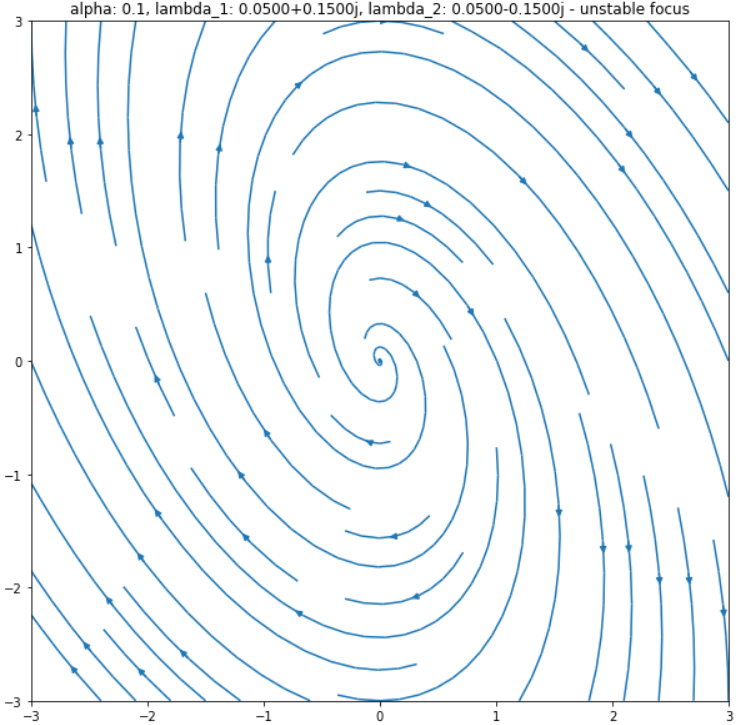
\includegraphics[width=0.3\textwidth]{images/unstable_focus.png}}
    \hfill
    \subfloat[b]{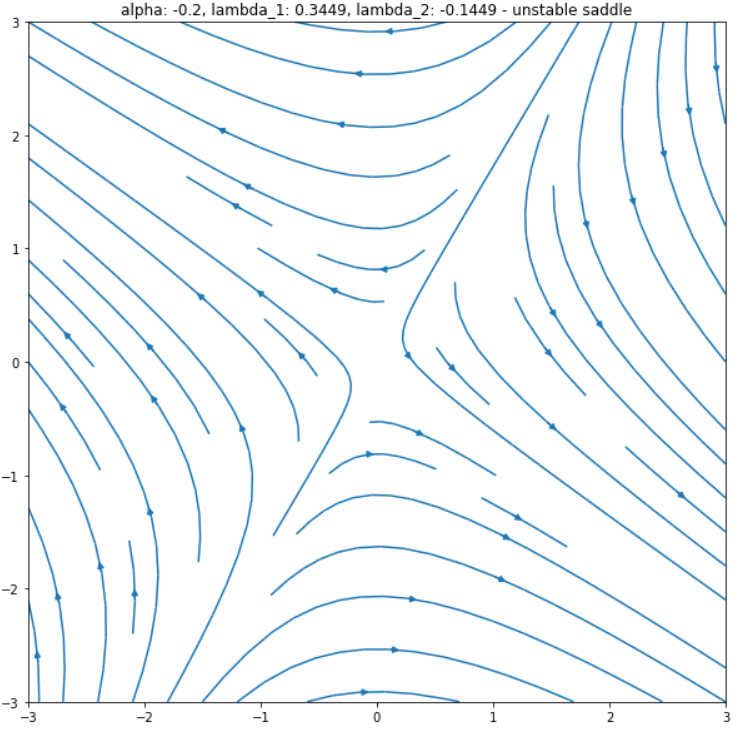
\includegraphics[width=0.3\textwidth]{images/unstable_saddle.png}}
    \hfill
    \subfloat[c]{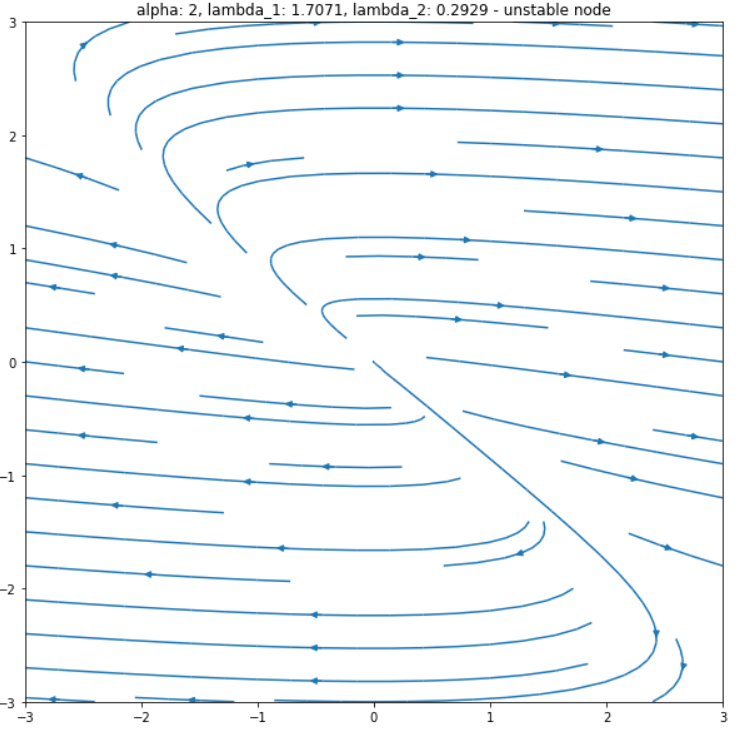
\includegraphics[width=0.3\textwidth]{images/unstable_node.png}}
    \vfill
    \subfloat[d]{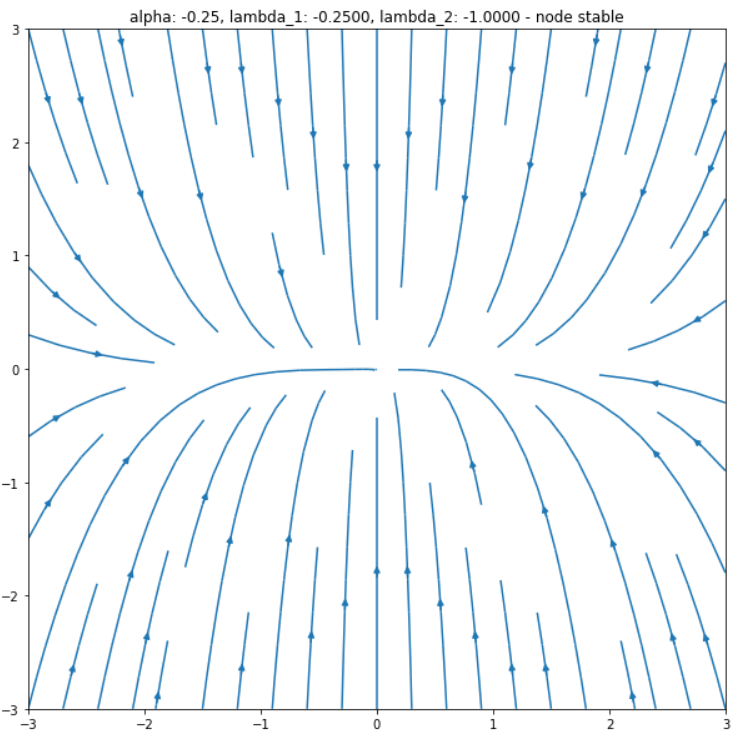
\includegraphics[width=0.3\textwidth]{images/stable_node.png}}
    \subfloat[e]{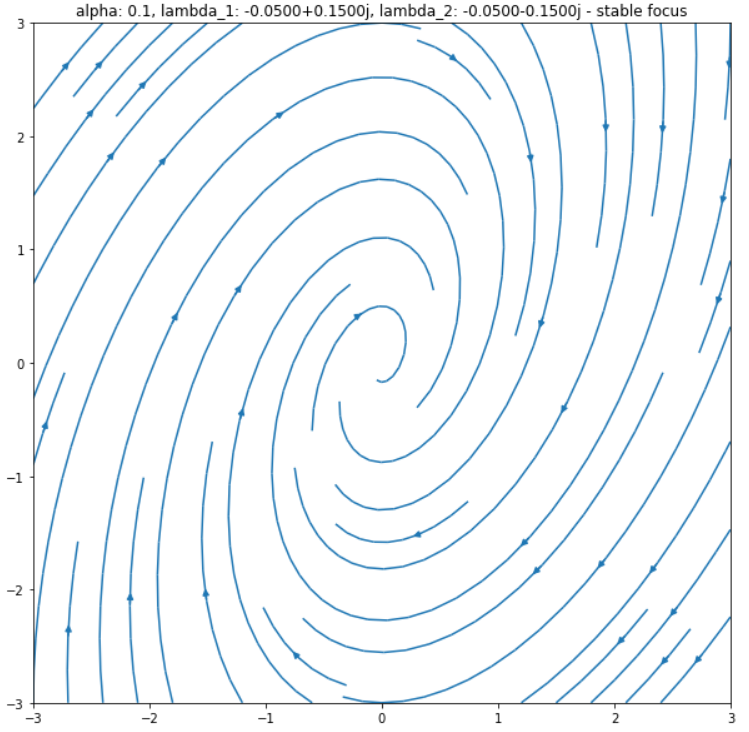
\includegraphics[width=0.3\textwidth]{images/stable_focus.png}}
    \caption{Phase portraits of task 1, namely:
    (a) Unstable focus;
    (b) Unstable saddle;
    (c) Unstable node;
    (d) Stable node;
    (e) Stable focus.}
    \label{fig:task1-phase-portraits}
\end{figure}
\end{task}


% TASK 2 -----------------------------------------------
\begin{task}{2, Common bifurcations in nonlinear systems}
This task asks for the analysis of the bifurcation for two dynamical systems: $$\dot x = \alpha - x^2$$ 
\begin{center}
    and
\end{center} $$\dot x = \alpha - 2x^2 - 3$$
The bifurcation diagrams for the two systems are described in \textbf{\hyperref[fig:task2]{Figure \ref{fig:task2}}}.


The two systems express a similar behaviour, with both having no steady state before a parametric value coincides with the \textit{bifurcation point} (e.g. $\alpha=0$ for the \textit{left} model). From then on the system has two different steady states. The bifurcation type for these two systems is called \textit{saddle-node bifurcation}, with one of the two steady states being repulsive and one attractive, colored in \textit{orange} and \textit{blue} in the \textbf{\hyperref[fig:task2]{Figure \ref{fig:task2}}}.

To answer the rest of the task questions it is relevant to cite (\cite{kuznetsov}, p.59): "\textit{For instance, it is natural to expect that two equivalent systems have the 
same number of equilibria and cycles of the same stability types. The "relative 
position" of these invariant sets and the shape of their regions of attraction 
should also be similar for equivalent systems.}".\\
Therefore it is safe to assert that the two systems are not topologically equivalent at $\alpha=1$ since the system on the \textit{left} has two steady states and system on the \textit{right} has no steady states. On the contrary, the two systems are topologically equivalent at $\alpha=-1$, since they have the same number of steady states and they actually have the same \textit{normal form}. One might hypothesize the two systems have the same normal form since their bifurcation diagrams are qualitatively equivalent and taking a look at the graphics there are some hints giving more proofs, using the two differences in the system (the $x^2$ coefficient and the $x^0$ coefficient):
\begin{itemize}
    \item the basic coefficient difference is having the $+3$ at the end of the equation, an element that simply delays the whole bifurcation. In fact the bifurcation point difference between the two systems is exactly $3$.
    \item the coefficient multiplying $x^2$ is simply changing the amplitude of the $y$ coordinate, stretching it by two times, which coincides with the multiplying coefficient, which is $2$.
\end{itemize}

It is therefore possible to obtain a mapping between the two dynamical systems, using a delay followed by a multiplication to map back the \textit{right} system into the \textit{left} one.


\begin{figure}[H]
    \centering
    \subfloat[a]{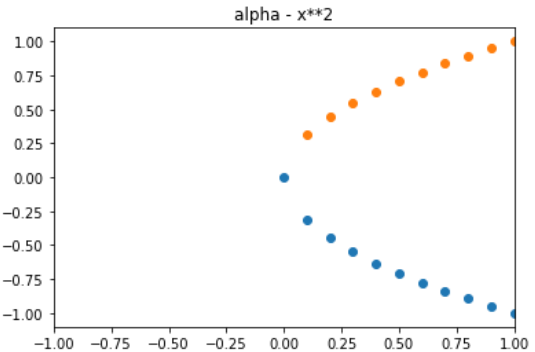
\includegraphics[width=0.45\textwidth]{images/task2_1.png}}\label{fig:task2_1}
    \hfill
    \subfloat[b]{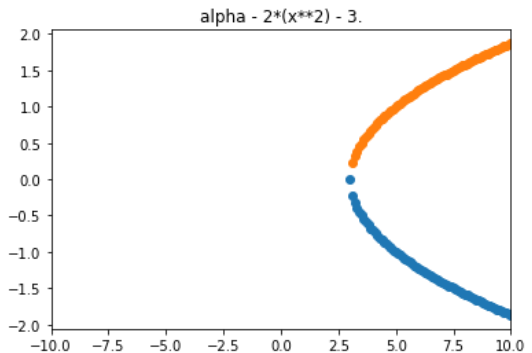
\includegraphics[width=0.45\textwidth]{images/task2_2.png}}\label{fig:task2_2}
    \caption{bifurcation diagrams for the two requested systems - \textit{alpha} on the x axis, \textit{x} coordinate on the y axis}
    \label{fig:task2}
\end{figure}

\end{task}


% TASK 3 -----------------------------------------------
\begin{task}{3, Bifurcations in higher dimensions} \label{sec:task3}
In this task an important bifurcation for systems with one parameter (but for two-dimensional state spaces) is analyzed: \textit{the Andronov-Hopf bifurcation}, representable with the vector field in normal form:
$$\dot x_1 = \alpha x_1 - x_2 - x_1(x_1^2 + x_2^2)$$
$$\dot x_2 = x_1 + \alpha x_2 - x_2(x_1^2 + x_2^2)$$

\paragraph{Task 3.1:}
The change in behaviour of such a system can be shown to intuitively understand the bifurcation that is happening. \textbf{\hyperref[fig:andronov-hopf-bifurcation]{Figure \ref{fig:andronov-hopf-bifurcation}}} gives three different portraits by varying the $\alpha$ parameter, specifically setting it to -1, 0 and 1:
\begin{itemize}
    \item for $\alpha=-1$ a single attractive stable point can be located in the origin.
    \item  for $\alpha=1$ an unstable point is located at the origin and a stable \textit{limit cycle} is present near the origin.
    \item for $\alpha=0$, as reported in \cite{kuznetsov} (p 85), a \textit{weekly attractive focus} is present in the origin. This parametric value represents the bifurcation point, moving from a stable fixed point to a limit cycle behaviour.
\end{itemize}
\begin{figure}[H]
    \centering
    \subfloat[a]{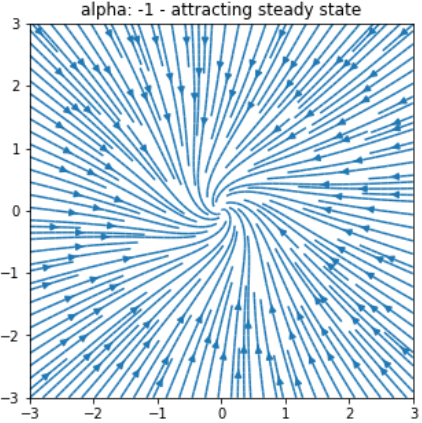
\includegraphics[width=0.3\textwidth]{images/phase-1.png}}
    \hfill
    \subfloat[b]{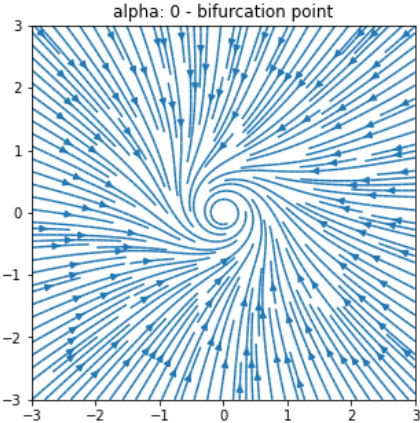
\includegraphics[width=0.3\textwidth]{images/phase0.png}}
    \hfill
    \subfloat[c]{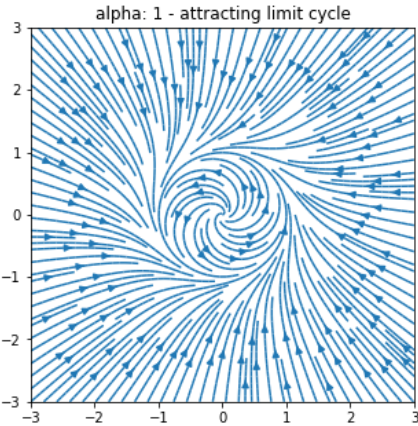
\includegraphics[width=0.3\textwidth]{images/phase1.png}}
    \caption{bifurcation shown three phase diagrams at representative values of $\alpha$.}
    \label{fig:andronov-hopf-bifurcation}
\end{figure}

\paragraph{Task 3.2:}
The second part of the task asks for the numerical computation and visualization of two orbits (starting at \textbf{[2, 0]} and \textbf{[0.5, 0]}) given a specific $\alpha$ value (in the requested case $\alpha=1$). The two requested orbits have been computed taking advantage of \textit{Euler's method}. Given the particular $\alpha$ value one should expect for any point not starting in the origin to converge to the limit cycle, either by repulsion from the origin or by attraction from outside the limit cycle.

\textbf{\hyperref[fig:plot-traj]{Figure \ref{fig:plot-traj}}} show the method implemented to perform the task, where different parameters gave the possibility of tuning the number of iterations as well as the time step for the algorithm. The core of the method is highlighted by the \textit{orange box}, where the two odes are assigned to be used by the underlying Euler's method step.
\begin{figure}[H]
    \centering
    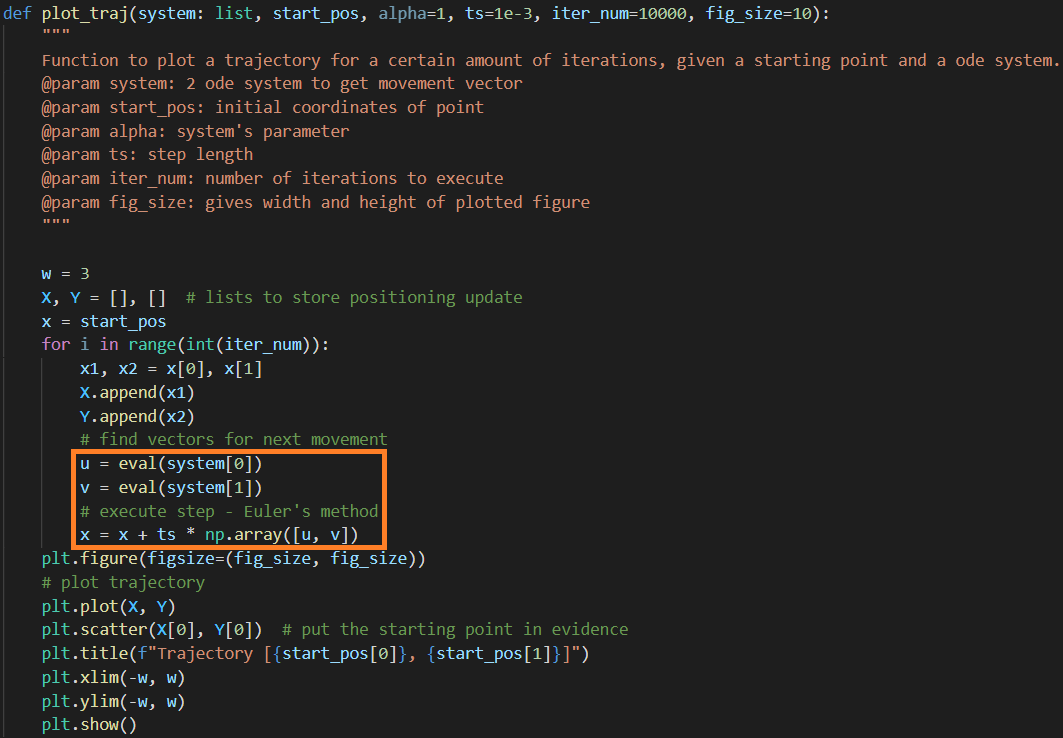
\includegraphics[scale=0.5]{images/plot_traj.png}
    \caption{snippet for trajectory plotting}
    \label{fig:plot-traj}
\end{figure}

Finally \textbf{\hyperref[fig:trajectories]{Figure \ref{fig:trajectories}}} plots the result, which follow the expectations. The blue dot denotes the starting point for each trajectory.
\begin{figure}[H]
    \centering
    \subfloat[a]{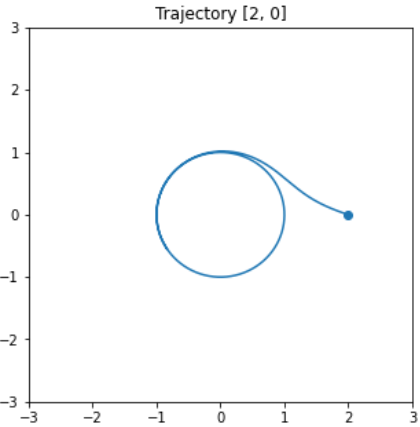
\includegraphics[width=0.3\textwidth]{images/traj0,2.png}}
    \hfill
    \subfloat[b]{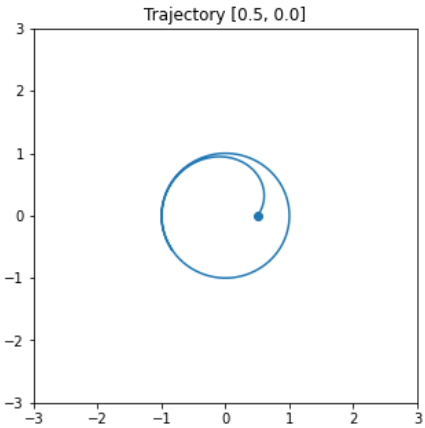
\includegraphics[width=0.3\textwidth]{images/traj05,0.png}}
    \caption{system orbits starting at point (2,0) and (0.5,0) for $\alpha = 1$}
    \label{fig:trajectories}
\end{figure}



\paragraph{Task 3.3:}
The last subtask asks for the analysis of a double parametered bifurcation, the \textit{cusp bifurcation}, with the following normal form:
$$\dot x = \alpha_1 + \alpha_2 x - x^3$$
Following the hint provided in the exercise sheet, the core snippet shown in \textbf{\hyperref[fig:cusp-code]{Figure \ref{fig:cusp-code}}} generates the data triples by first sampling $\alpha_2$ and $x$ values, to then compute the relative $\alpha_1$ values by reversing the normal form (we know that a fixed point is a point such that $\dot x = 0$). 

\begin{figure}[H]
    \centering
    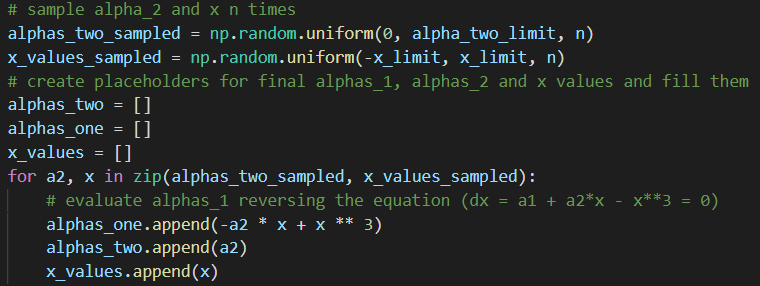
\includegraphics[scale=1]{images/cusp_bifurc.png}
    \caption{\textit{cusp} implementation core snippet}
    \label{fig:cusp-code}
\end{figure}

The 3D plot of such a system (with an adequate colormap to try and highlight better the surface shape) is shown in \textbf{\hyperref[fig:cusp-3d]{Figure \ref{fig:cusp-3d}}} from two different points of view. An \textit{hysteresis phenomenon} is visible and is responsible for the cusp generation. 

\begin{figure}[H]
    \centering
    \subfloat[a]{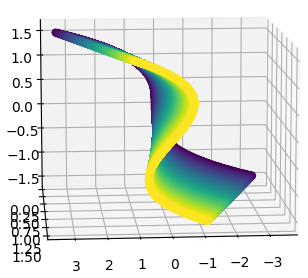
\includegraphics[width=0.4\textwidth]{images/cusp3d1.png}}
    \hfill
    \subfloat[b]{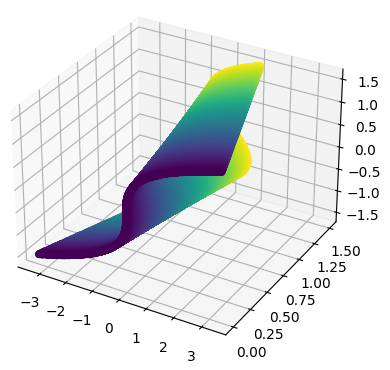
\includegraphics[width=0.4\textwidth]{images/cusp3d2.png}}
    \caption{\textit{cusp} bifurcation system in 3D from 2 different angulations}
    \label{fig:cusp-3d}
\end{figure}
\end{task}

The bifurcation gets his name in fact by the presence of a \textit{cusp} shape when projecting the $x$ dimension in the $\alpha_1$ and $\alpha_2$ plane. The particular surface shown in \textbf{\hyperref[fig:cusp-3d]{Figure \ref{fig:cusp-3d}}} does in fact imply that for a given ($\alpha_1$, $\alpha_2$) configuration there can be one or more than one steady states, implying a bifurcation. In \textbf{\hyperref[fig:cusp-projection]{Figure \ref{fig:cusp-projection}}} is shown a projection where coordinates with multiple $x$ values are shown in \textit{orange} and ones with only one value are shown in \textit{blue}. To achieve such a feat the alphas values coming out of the snippet shown in \textbf{\hyperref[fig:cusp-code]{Figure \ref{fig:cusp-code}}} have been rounded to overcome floating point granularity not giving the expected result. This procedure was nevertheless not flawless, bringing also some noise due to the original value sampling fused with the rounding previously explained.

\begin{figure}[H]
    \centering
    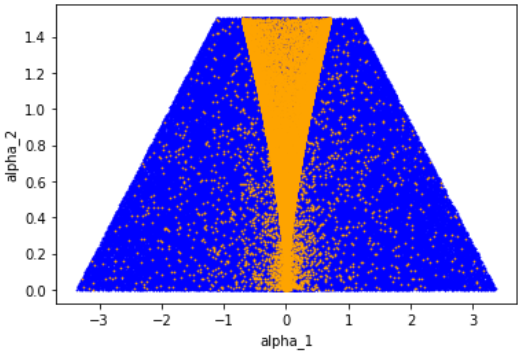
\includegraphics[scale=1]{images/cusp.png}
    \caption{\textit{cusp} projection on the alpha space}
    \label{fig:cusp-projection}
\end{figure}


% TASK 4 -----------------------------------------------
\begin{task}{4, Chaotic dynamics}
In this task we analyze some aspects of the \textit{logistic map} system, expressed by the following discrete map:
\begin{equation}\label{eq:logistic-map}
    x_{n+1} = r x_n (1 - x_n)
\end{equation}
with $x_n \in \mathbb{R},\ n \in \mathbb{N}$ and $r \in (0, 4]$.\\
To analyze this system, we created some helping functions that have been put in the script \texttt{utilities.py}, in particular:
\begin{itemize}
    \item \texttt{logistic}: computes the new state $x_{n+1}$ of the system (\hyperref[eq:logistic-map]{Eq. \ref{eq:logistic-map}}) given the current state $x_n$ and the $r$ parameter.
    
    \item \texttt{plot\_logistic\_map\_bifurcations}: takes 2 values of the parameter $r$ - a minimum ($r_m{min}$) and a maximum one ($r_{max})$ - and plots the behavior of the system of Eq. \ref{eq:logistic-map} $\forall r \in [r_{min},\ r_{max}]$.\\
    To do this, the system is run $n$ times for $m$ iterations, of which, only the last $p$ values are kept.
    This because, starting from an initial point $x_0$, the system will need a certain number of steps to reach a steady state, and since the objective of this plot is to show the steady states associated to different values of $r$, all the states assumed by the system in this initial phase are not of interest, and are therefore discarded.\\
    Note: we do not keep only the last state assumed by the system during the $m$ iterations because the system may find itself in a limit cycle or in a chaotic behaviour, therefore it is needed to have more than 1 value to see if there are a certain number of recurrent states associated to a certain value of $r$.\\
    The code of this function is shown in \hyperref[fig:plot-logistic-map-bifurcations]{Figure \ref{fig:plot-logistic-map-bifurcations}}.
    
    \item \texttt{logistic\_map\_cobweb\_plot}: shows the cobweb plot, which is a tool used to investigate the qualitative behavior of one-dimensional iterated functions, such as the logistic map \cite{cobweb}.
\end{itemize}

\begin{figure}[t]
    \centering
    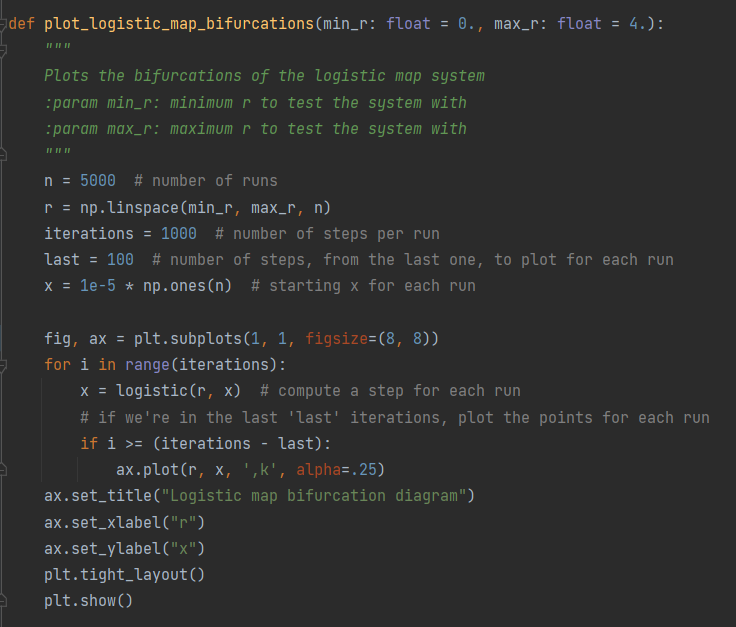
\includegraphics[scale=0.8]{images/code-plot_logistic_map_bifurcations.png}
    \caption{Code of the function \texttt{plot\_logistic\_map\_bifurcations}}
    \label{fig:plot-logistic-map-bifurcations}
\end{figure}

\paragraph{Task 4.1:}
By varying $r$ from 0 to 2, the bifurcation diagram obtained with the function \texttt{plot\_logistic\_map\_bifurcations} illustrated previously is shown in Figure \hyperref[fig:logistic-bifurcs]{\ref{fig:logistic-bifurcs}(a)}.\\
It is possible to see that there is one steady state for each value of $r$, in particular:
\begin{itemize}
    \item $r \in (0,\ 1] \implies x = 0$
    \item $r \in (1,\ 2] \implies x = \frac{r - 1}{r}$
\end{itemize}
In this case, there is no bifurcation and the steady state of the system is always one ($\forall r \in (0, 2]$).
This fixed point is attractive, because, since each point in the bifurcation diagram is obtained plotting the last $p$ states assumed by the system for a certain value of $r$, if the steady state in object was repulsive, we would have multiple points per value of $r$, instead this is not the case.\\
Furthermore, in the cobweb plot in Figure \ref{fig:cobweb-4.1} it is possible to see how the system tends to a certain steady state: 0 for $r = 0.8$, 0.44 for $r = 1.8$.

\begin{figure}[b]
    \centering
    \subfloat[a]{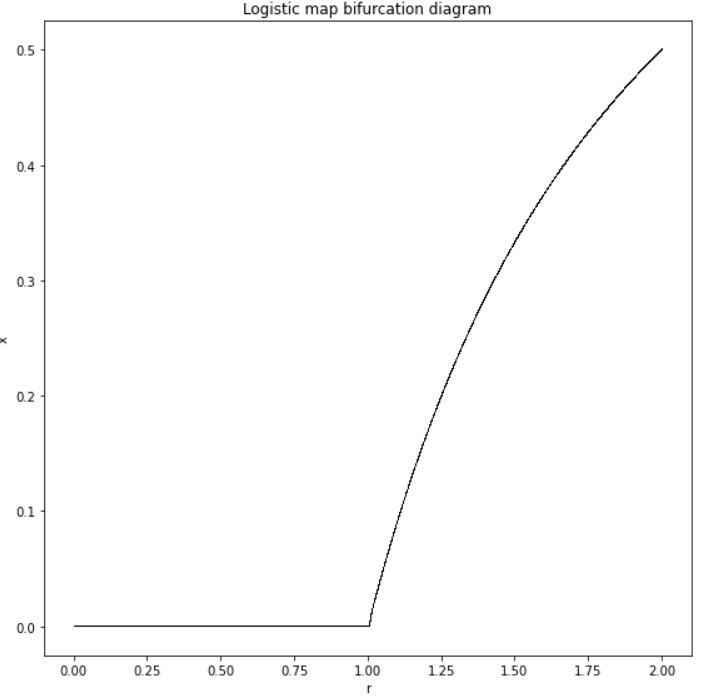
\includegraphics[width=0.3\textwidth]{images/logistic_bifurc_r0-2.png}}
    \hfill
    \subfloat[b]{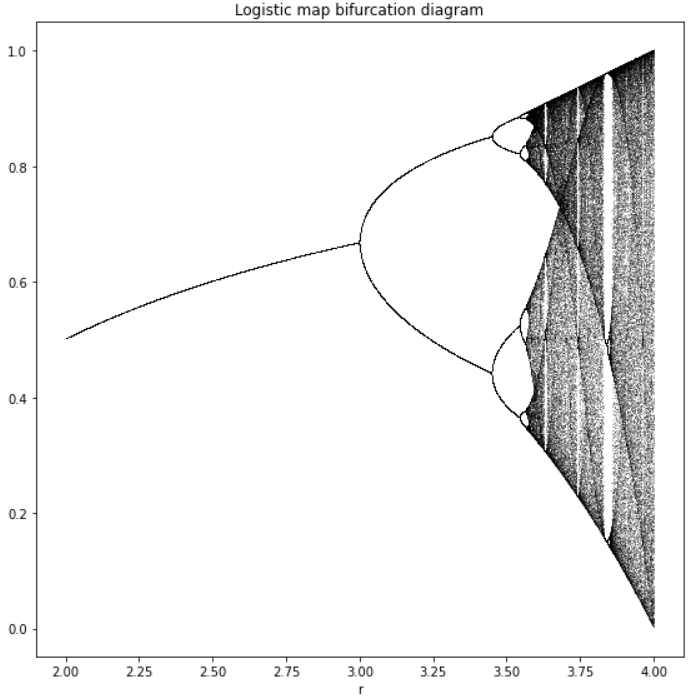
\includegraphics[width=0.3\textwidth]{images/logistic_bifurc_r2-4.png}}
    \hfill
    \subfloat[c]{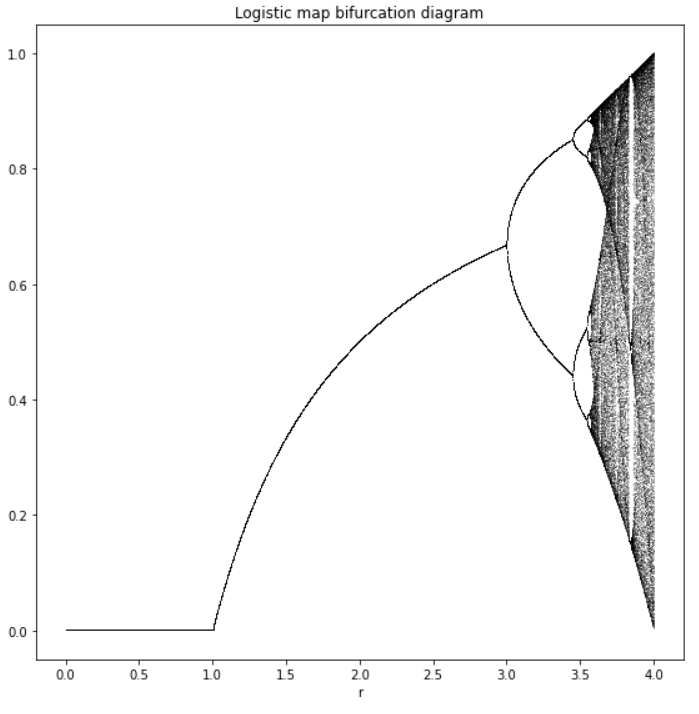
\includegraphics[width=0.3\textwidth]{images/logistic_bifurc_r0-4.png}}
    \caption{Bifurcations of the logistic map with:
    $r \in (0,\ 2]$ (a);
    $r \in [2, 4]$ (b);
    $r \in (0, 4]$ (c).}
    \label{fig:logistic-bifurcs}
\end{figure}

\begin{figure}[t]
    \centering
    \subfloat[a]{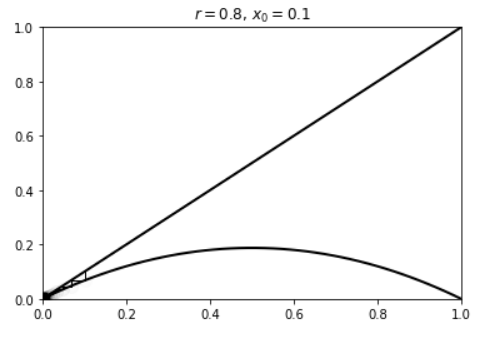
\includegraphics[width=0.45\textwidth]{images/cobweb_r0.8.png}}
    \hfill
    \subfloat[b]{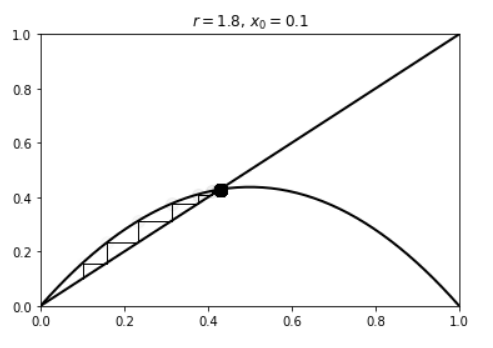
\includegraphics[width=0.45\textwidth]{images/cobweb_r1.8.png}}
    \caption{Cobweb plot with (a) $r = 0.8$ and (b) $r = 1.8$.}
    \label{fig:cobweb-4.1}
\end{figure}

\paragraph{Task 4.2:}
Varying $r$ from 2 to 4, the number of steady states continue to double more and more often, with the exceptions of few stability islands.
This behavior is shown in Figure \ref{fig:logistic-bifurcs}(b).
Moreover, Figure \ref{fig:cobweb-4.2} shows the various limit cycles with an increasing number of steady states as $r$ increases.

\begin{figure}[H]
    \centering
    \subfloat[a]{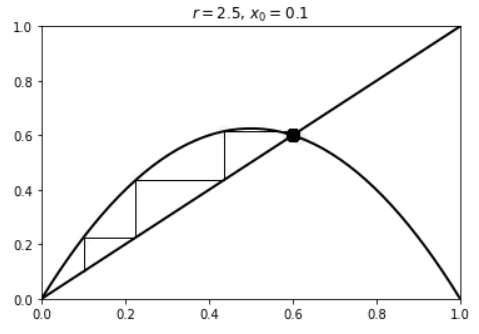
\includegraphics[width=0.3\textwidth]{images/cobweb_r2.5.png}}
    \hfill
    \subfloat[b]{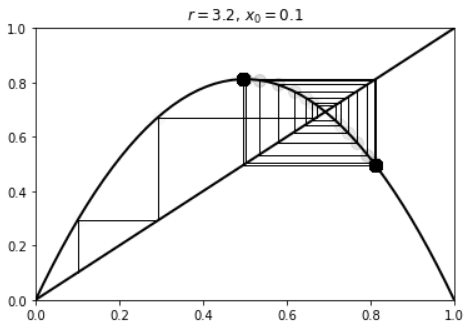
\includegraphics[width=0.3\textwidth]{images/cobweb_r3.2.png}}
    \hfill
    \subfloat[c]{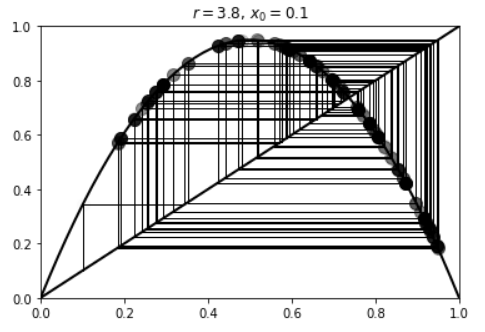
\includegraphics[width=0.3\textwidth]{images/cobweb_r3.8.png}}
    \caption{Cobweb plot with (a) $r = 2.5$, (b) $r = 3.2$ and (c) $r = .8$.}
    \label{fig:cobweb-4.2}
\end{figure}

\paragraph{Task 4.3:}
Figure \hyperref[fig:logistic-bifurcs]{\ref{fig:logistic-bifurcs}(c)} shows the bifurcations of the logistic map for $r \in (0,\ 4]$.
\begin{itemize}
    \item $\forall r \in (0,\ 1]:\ x = 0$ is a steady state
    \item $\forall r \in (1,\ 3):\ x = \frac{r-1}{r}$ is a steady state
    \item $\forall r \geq 3$ there are limit cycles that include a different number of points, initially an oscillation between two states, then at roughly 3.4 the oscillation becomes between four states.
    This number tend to increase (doubling) as $r$ increases, until at approximately $r=3.57$ the behaviour becomes chaotic with some exceptions being sporadic stability islands where once again oscillation between a little number of states is present.
\end{itemize}

\paragraph{Part 2 - Lorenz attractor:}
The focus of this part is to analyze the \textit{Lorenz attractor} \cite{lorenz}.
The system is defined as follows:
\begin{equation}\label{eq:lorenz}
    \begin{split}
        &\frac{\partial x}{\partial t} = \sigma(y - x)\\
        &\frac{\partial y}{\partial t} = x(\rho - z) - y\\
        &\frac{\partial z}{\partial t} = x y - \beta z
    \end{split}
\end{equation}
where $x,\ y$ and $z$ represent the coordinates of a point/state of the system, while $\sigma,\ \rho$ and $\beta$ are parameters.\\
The system has been simulated for 1000 seconds and its trajectory has been plotted.
Specifically, starting from $x_0 = (10,\ 10,\ 10)$ we obtain the plot depicted in Figure \hyperref[fig:lorenz-trajs-1000s]{\ref{fig:lorenz-trajs-1000s}(a)}, while \hyperref[fig:lorenz-trajs-1000s]{\ref{fig:lorenz-trajs-1000s}(b)} shows the plot starting from $\hat{x}_0 = (10+10^{-8},\ 10,\ 10)$.
In both cases the parameters were set to $\sigma = 10,\ \beta = 8/3,\ \rho = 28$.\\
Since the image is a little dense, simulations have been run with the same configurations but for 200 seconds instead of 1000.
This is shown in Figure \ref{fig:lorenz-trajs-200s}.\\
Since the system is chaotic, the minimal perturbation in the starting point (going from $x_0$ to $\hat{x}_0$) is visible on a macroscopic scale when plotting the trajectory of the system starting from that point.
The difference between the two trajectories, expressed as $\|x(t)-\hat{x}(t)\|^2\ \forall t$, is shown in Figure \ref{fig:lorenz-trajs-differences}, where it is possible to notice how this difference assumes relatively large values.
Specifically, this distance becomes larger than 1 after 13.48 seconds.

\begin{figure}[H]
    \centering
    \subfloat[a]{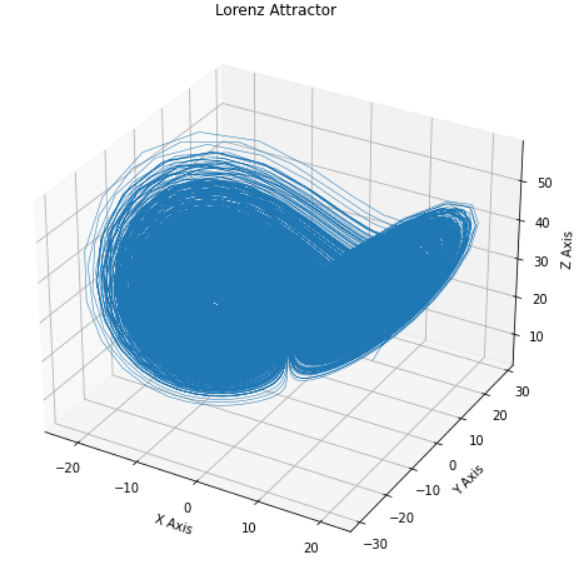
\includegraphics[width=0.45\textwidth]{images/lorenz_traj_10-10-10.png}}
    \hfill
    \subfloat[b]{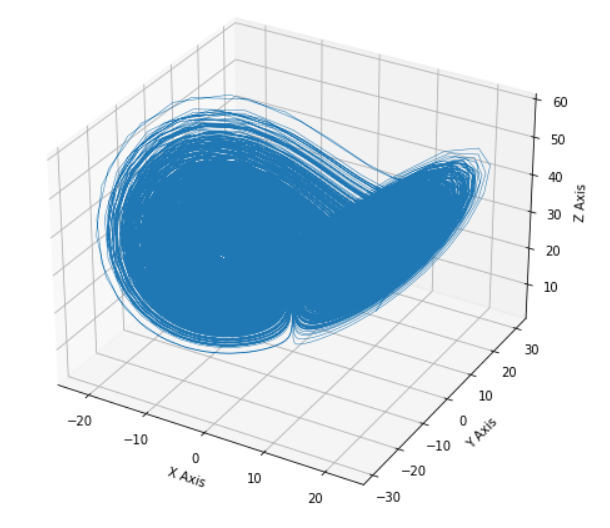
\includegraphics[width=0.45\textwidth]{images/lorenz_traj_10-10-10_perturbed.png}}
    \caption{Trajectories of the \textit{Lorenz attractor} simulated for 1000 seconds, starting from (a) $x_0 = (10,\ 10,\ 10)$ and (b) $\hat{x}_0 = (10+10^{-8},\ 10,\ 10)$ with $\sigma = 10,\ \beta = 8/3,\ \rho = 28$.}
    \label{fig:lorenz-trajs-1000s}
\end{figure}

\begin{figure}[H]
    \centering
    \subfloat[a]{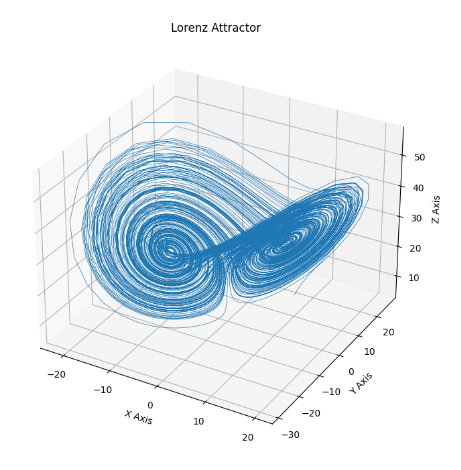
\includegraphics[width=0.45\textwidth]{images/lorenz_traj_10-10-10_200s.png}}
    \hfill
    \subfloat[b]{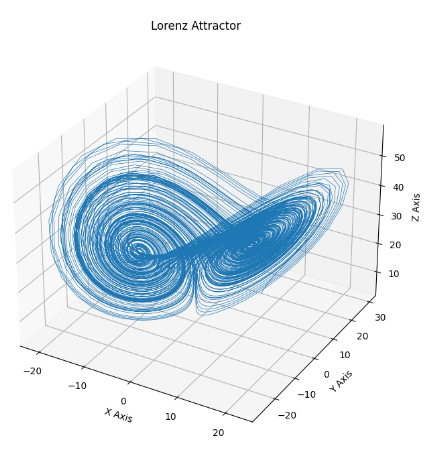
\includegraphics[width=0.45\textwidth]{images/lorenz_traj_10-10-10_perturbed_200s.png}}
    \caption{Trajectories of the \textit{Lorenz attractor} simulated for 200 seconds, starting from (a) $x_0 = (10,\ 10,\ 10)$ and (b) $\hat{x}_0 = (10+10^{-8},\ 10,\ 10)$ with $\sigma = 10,\ \beta = 8/3,\ \rho = 28$.}
    \label{fig:lorenz-trajs-200s}
\end{figure}

\begin{figure}[H]
    \centering
    \subfloats[a]{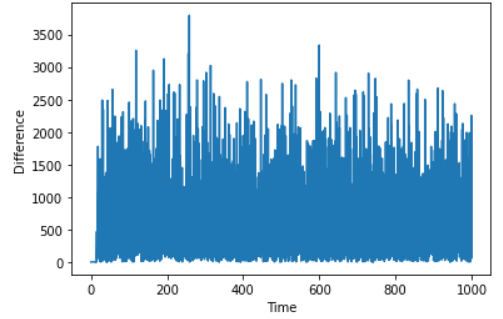
\includegraphics[width=0.45\textwidth]{images/lorenz_trajs_differences.png}}
    \hfill
    \subfloats[a]{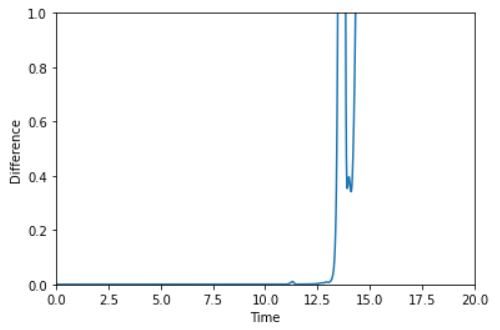
\includegraphics[width=0.45\textwidth]{images/lorenz_trajs_differences_closeup.png}}
    \caption{The difference between the trajectory of the \textit{Lorenz attractor} starting from $x_0=(10,\ 10,\ 10)$ and $\hat{x}_0=(10+19^{-8},\ 10,\ 10)$.
    For each value $t$ on the x-axis the plot shows $\|x(t)-\hat{x}(t)\|^2$.\\
    (b) shows simply a close-up of (a): the plot is the same but the x and y axes have been shortened.}
    \label{fig:lorenz-trajs-differences}
\end{figure}

Now, setting $\rho = 0.5$ and repeating these tests, it is possible to observe in Figure \ref{fig:lorenz-trajs-1000s-r0.5} that the trajectories are identical to each other, but very different from before, indicating that a bifurcation occurs for a certain value of $\rho$ between 0.5 and 28.

\begin{figure}[H]
    \centering
    \subfloat[a]{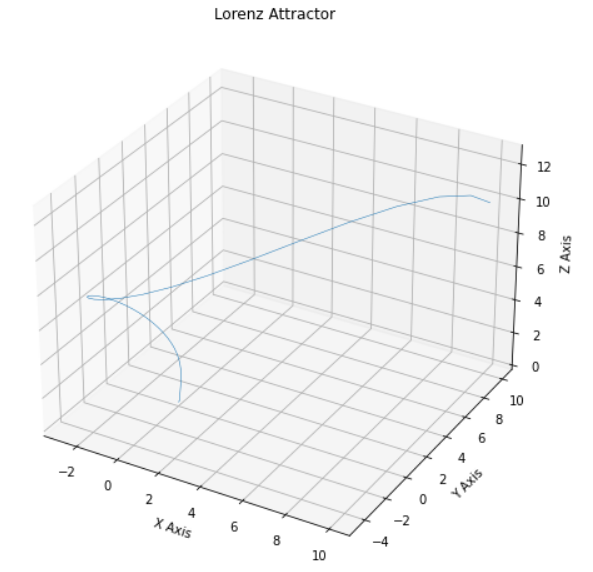
\includegraphics[width=0.45\textwidth]{images/lorenz_traj_10-10-10_r0.5.png}}
    \hfill
    \subfloat[b]{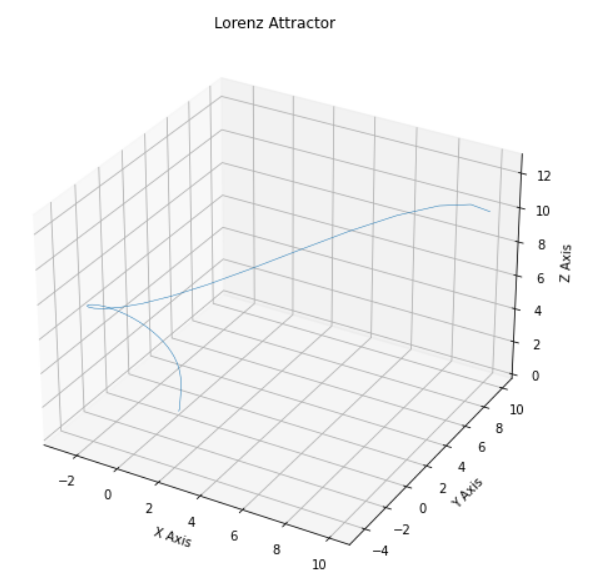
\includegraphics[width=0.45\textwidth]{images/lorenz_traj_10-10-10_perturbed_r0.5.png}}
    \caption{Trajectories of the \textit{Lorenz attractor} simulated for 1000 seconds, starting from (a) $x_0 = (10,\ 10,\ 10)$ and (b) $\hat{x}_0 = (10+10^{-8},\ 10,\ 10)$ with $\sigma = 10,\ \beta = 8/3,\ \rho = 0.5$.}
    \label{fig:lorenz-trajs-1000s-r0.5}
\end{figure}

\end{task}


\begin{task}{5, Bifurcations in crowd dynamics}
\paragraph{Task 5.1 - 5.2:}
The Jupyter notebook \texttt{sir\_bed\_mode\_unfinished.ipynb}, as the name suggests, is not complete.
The main aspect that had to be addressed is the fact that the equations that define the SIR model are not implemented (\hyperref[fig:sir-eqq-code]{Figure \ref{fig:sir-eqq-code}}).
It was straight forward to implement those equations having all the parameters needed (passed as arguments to the function): $\mu_0,\ \mu_1,\ \beta,\ A,\ d,\ \nu$ and $b$.\\
Other than that all the functions present in the notebook (namely \texttt{mu}, \texttt{R0}, \texttt{h} and \texttt{model}) have been moved to a new script called \texttt{sir\_utilities.py}.
Furthermore some code present in the notebook - for example the one to plot the system's trajectories and the behavior of the 3 variables (S, I, R) over time - has been put in specific functions placed in the new script to make everything more modular, tidy and reusable.\\
As a final point, the documentation has been improved or added when (partially) missing.

\begin{figure}[H]
    \centering
    \subplots[a]{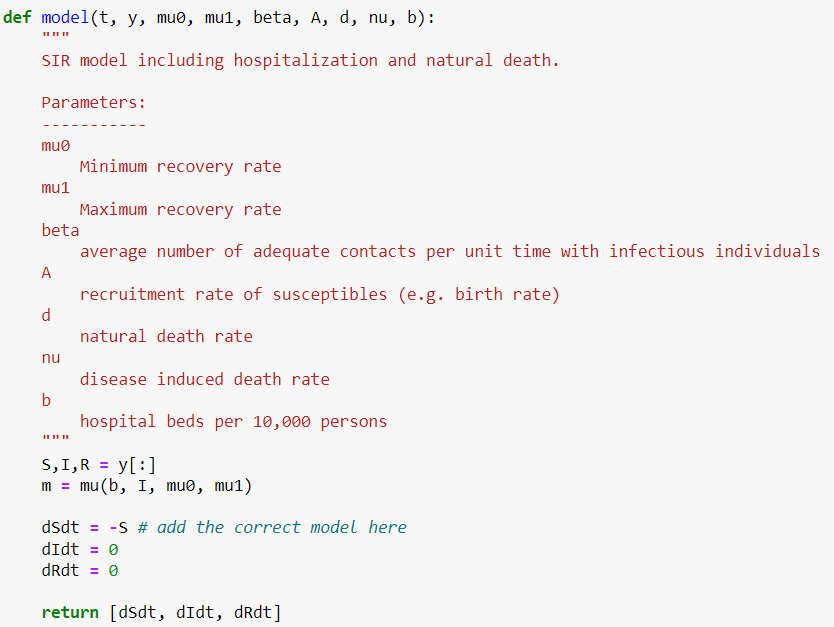
\includegraphics[width=0.45\textwidth]{images/code_SIR_eqq_unfinished.png}}
    \hfill
    \subplots[b]{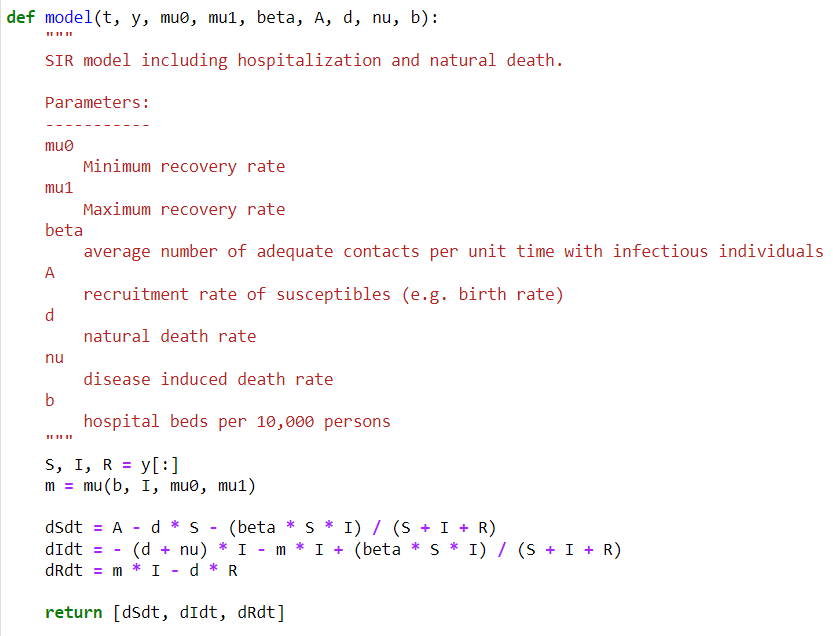
\includegraphics[width=0.45\textwidth]{images/code_SIR_eqq_finished.png}}
    \caption{The code implementing the SIR model's equations. (a) the unfinished code given in the example notebook; (b) the completed code.}
    \label{fig:sir-eqq-code}
\end{figure}

\paragraph{Task 5.3:}
The parameterized proposed scenario follows the ruled behaviour described in \textbf{\hyperref[kuznetsov]{\cite{kuznetsov}, Section 4}}, where the study of  parameterized models being non \textit{globally asymptotically stable} in $E_0$ is carried out. $E_0$ is in our case the initial condition [200, 0, 0] and our parameterized system is non \textit{globally asymptotically stable} in that point since $R0 < 1$ (0.99) and $\beta > d + \nu + \mu_0$ ($11.5 > 11.1$). 

The scenario does therefore produce a bifurcation when varying the \texttt{b} parameter, as graphically portrayed in \textbf{\hyperref[fig:sir-bifurcation]{Figure \ref{fig:sir-bifurcation}}}.
What is represented in the aforementioned figure is a trajectory plotting by varying \texttt{b} in the range $(0.01, 0.03)$ (with 0.001 as step), with each subfigure showing the trajectory of three different initial points:
\begin{itemize}
    \item first point is initiated with \textbf{[195.3, 0.052, 4.4]} as SIR values. Its trajectory is colored in \textbf{red} and its initial (\textbf{x symbol}) and final (\textbf{romboid symbol}) trajectory landmarks are colored in \textbf{black}.
    \item second point is initiated with \textbf{[195.7, 0.03, 3.92]} as SIR values. Its trajectory is colored in \textbf{green} and its initial (\textbf{x symbol}) and final (\textbf{romboid symbol}) trajectory landmarks are colored in \textbf{light violet}.
    \item last point is initiated with \textbf{[193, 0.08, 6.21]} as SIR values. Its trajectory is colored in \textbf{blue} and its initial (\textbf{x symbol}) and final (\textbf{romboid symbol}) trajectory landmarks are colored in \textbf{orange}.
\end{itemize}
To discuss the behaviour change when increasing \texttt{b}:
\begin{itemize}
    \item for \textbf{$b < 0.022$} the system shows a local attractive point in [193.666, 0.057, 5.71] for the three points in consideration, resembling ever more a stable focus as $b$ increases in value (\textbf{\hyperref[fig:sir-bifurcation]{Figure \ref{fig:sir-bifurcation}}.c-d}). 
    \item at \textbf{$b = 0.022$} the system encounters its bifurcation point, with [193.666, 0.057, 5.71] being a weak stable point since it is attracting the nearest point (the red plot) while a new behaviour shows up, with the other two points being attracted to a limit cycle (\textbf{\hyperref[fig:sir-bifurcation]{Figure \ref{fig:sir-bifurcation}}.f}). In particular the limit cycle is attractive both from the inside (the green plot) and from the outside (the blue plot). 
    \item for \textbf{$b > 0.022$} the system slowly converges once again to having an attractive steady state, which is actually $E_0$ [200, 0, 0] (\textbf{\hyperref[fig:sir-bifurcation]{Figure \ref{fig:sir-bifurcation}}.g-h}).
\end{itemize}
Just to address it, \textbf{\hyperref[fig:sir-bifurcation]{Figure \ref{fig:sir-bifurcation}}} is composed of 2D images since 3D images such as the one portrayed in \textbf{\hyperref[fig:sir-bifurcation-3d]{Figure \ref{fig:sir-bifurcation-3d}}} do in our opinion make it harder to visualize single points while not adding much more qualitative information with respect to 2D.
\begin{figure}[h]
    \centering
    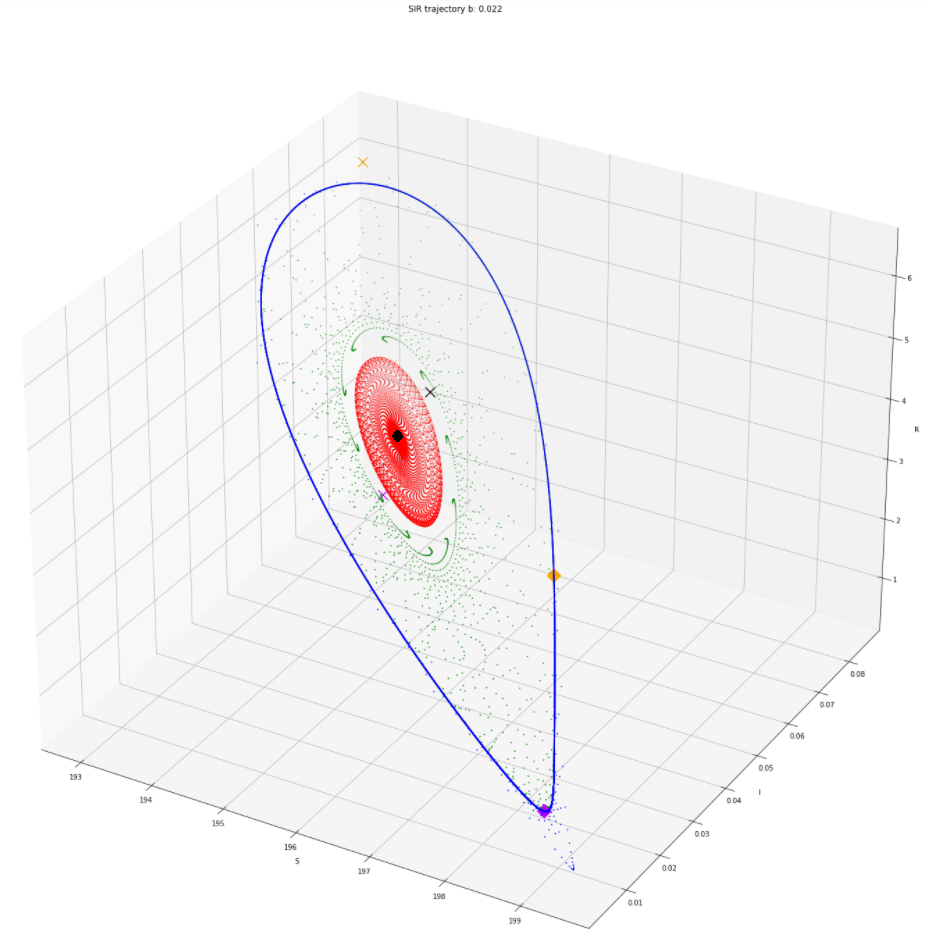
\includegraphics[scale=0.32]{images/5.3.big.png}
    \caption{bifurcation point in 3D}
    \label{fig:sir-bifurcation-3d}
\end{figure}

\pagebreak
\begin{figure}[ht!]
 \centering
 \subfloat[a]{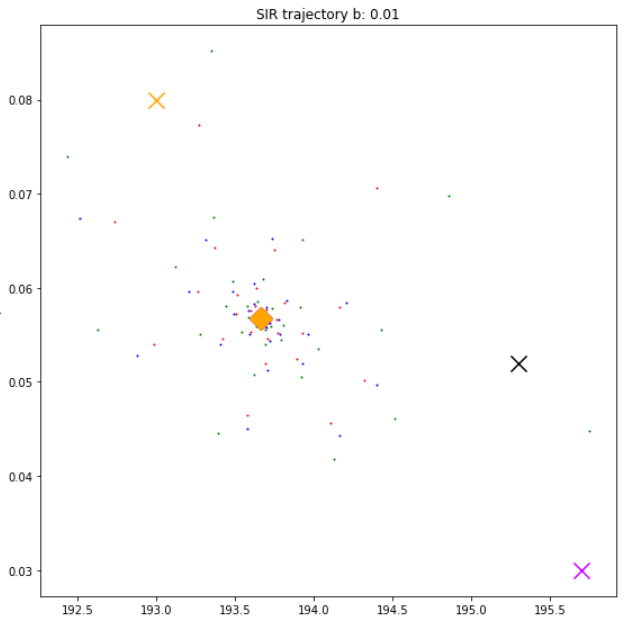
\includegraphics[width=0.32\textwidth]{images/5.3.1.png}}%
 \subfloat[b]{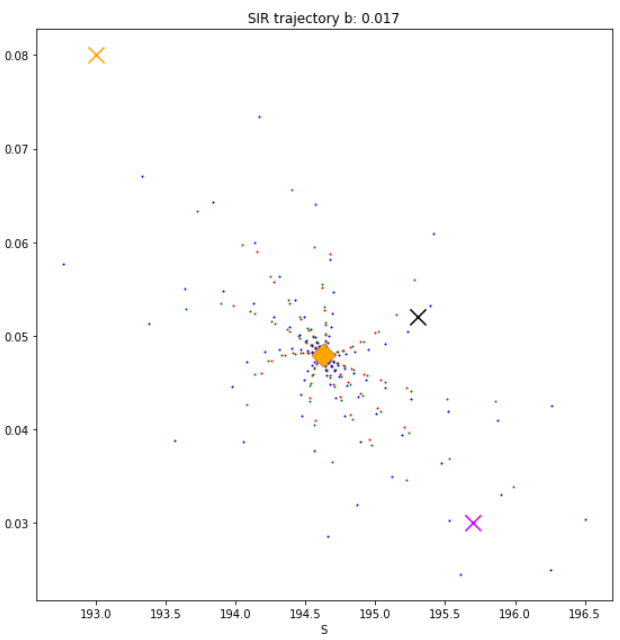
\includegraphics[width=0.32\textwidth]{images/5.3.2.png}}%
 \subfloat[c]{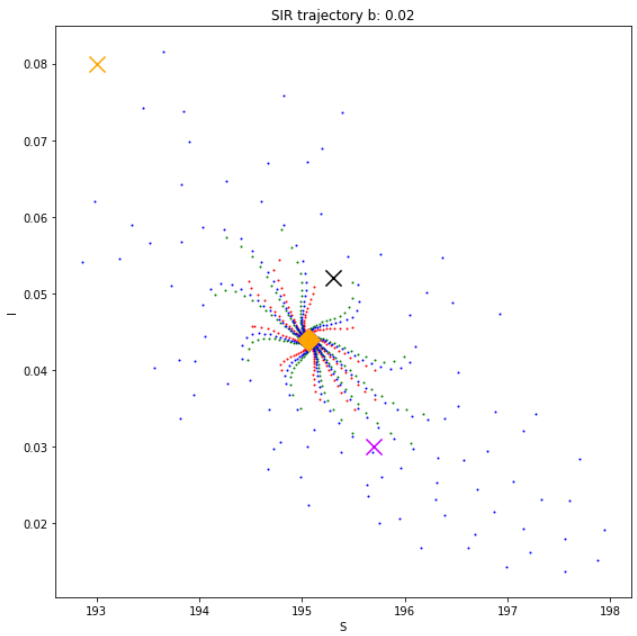
\includegraphics[width=0.32\textwidth]{images/5.3.3.png}}\\
 \subfloat[d]{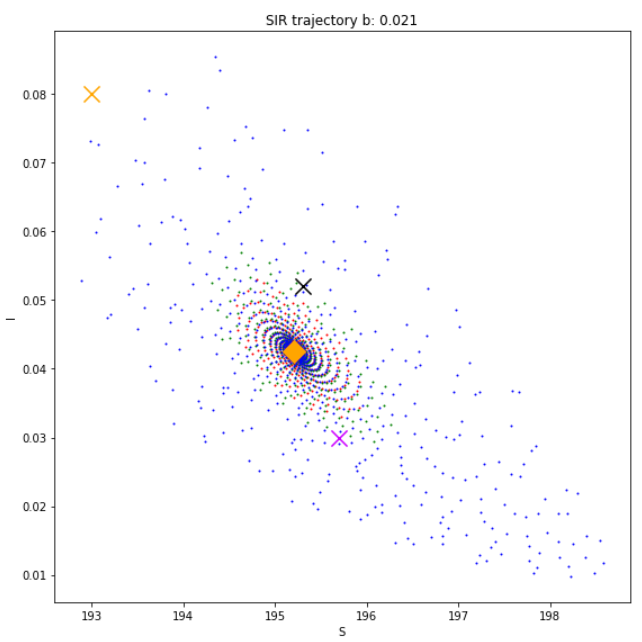
\includegraphics[width=0.32\textwidth]{images/5.3.4.png}}%
 \subfloat[e]{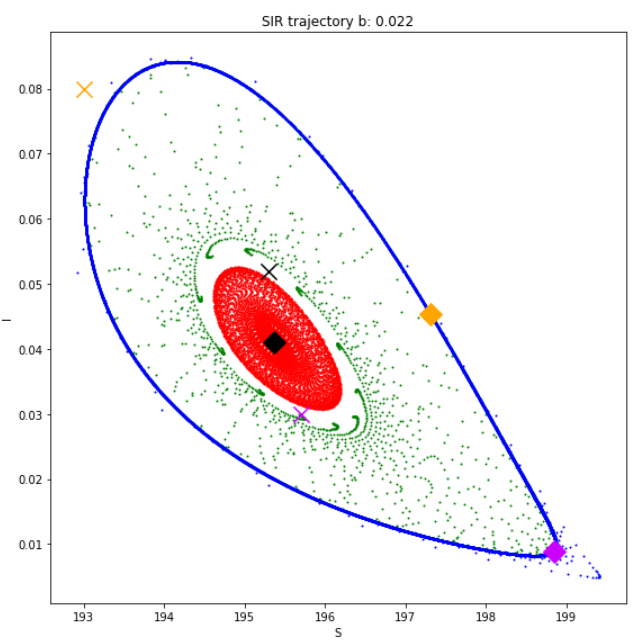
\includegraphics[width=0.32\textwidth]{images/5.3.5.png}}%
 \subfloat[f]{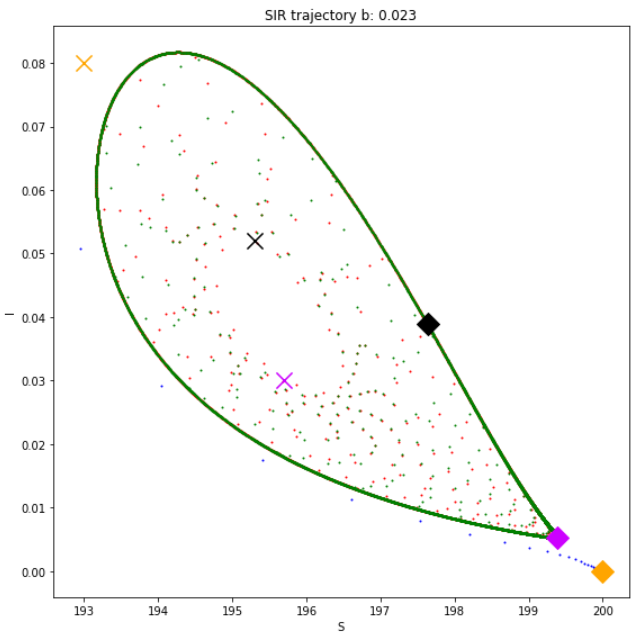
\includegraphics[width=0.32\textwidth]{images/5.3.6.png}}\\
 \subfloat[g]{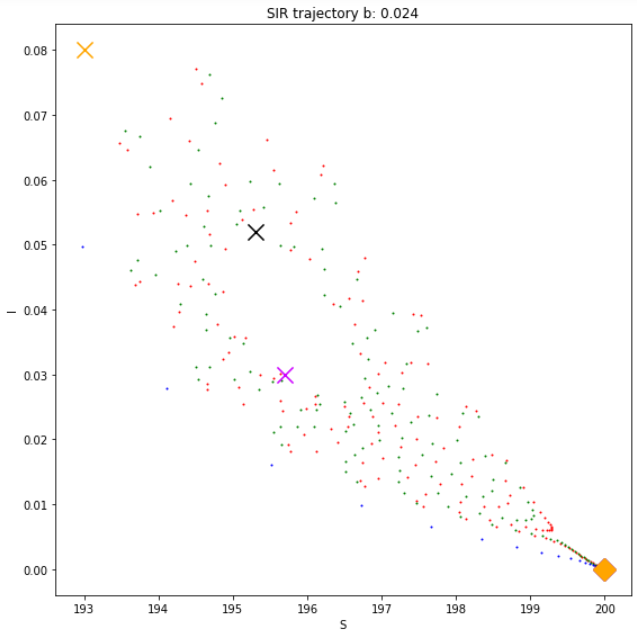
\includegraphics[width=0.32\textwidth]{images/5.3.7.png}}%
 \subfloat[h]{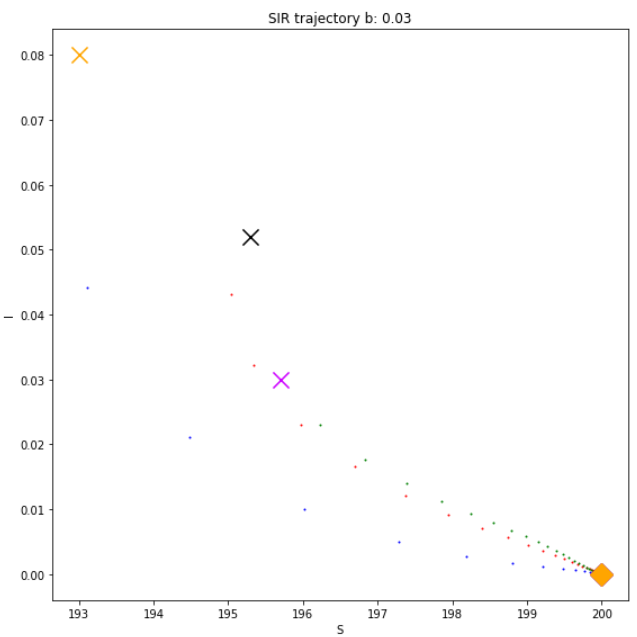
\includegraphics[width=0.32\textwidth]{images/5.3.8.png}}%
 \caption{showing SIR behaviour change by varying \texttt{b} - time evolution from left to right and up to down}%
 \label{fig:sir-bifurcation}%
\end{figure}
\pagebreak



\paragraph{Task 5.4:}
The bifurcation shown in the previous paragraph appears at $b = 0.022$. Following the \textbf{Lemma 4.3} in \cite{kuznetsov} it is possible to demonstrate it is a \textit{Hopf Bifurcation}, going locally from a steady state to a limit cycle as we previously have seen in \textbf{\hyperref[sec:task3]{Section Task 3}}. The calculations are shown in file \texttt{EX3/task5.ipynb} following the lemma conditions. Eventually, the normal form is the one mentioned in the same aforementiond section:
$$\dot x_1 = \alpha x_1 - x_2 - x_1(x_1^2 + x_2^2)$$
$$\dot x_2 = x_1 + \alpha x_2 - x_2(x_1^2 + x_2^2)$$

\paragraph{Task 5.5:}
The \textit{basic reproduction number} is defined in \cite{SHAN20141662} as:
\begin{equation}
    \mathbb{R}_0 = \frac{\beta}{d + \nu + \mu_1}\ .
\end{equation}
Therefore, the variables used to compute it are $\beta,\ d,\ \nu$ and $\mu_1$, and they represent respectively the average number of contacts per unit of time with infectious people ($\beta$), the natural death rate per capita (d), the disease-induced death rate per capita ($\nu$) and the maximum recovery rate (dependant of the number of available hospital beds) ($\mu_1$).
% \footnote{$\beta$: the average number of contacts per unit of time with infectious people;\\
% d: per capita natural death rate;\\
% $\nu$: per capita disease-induced death rate;\\
% $\mu_1$: maximum recovery rate (dependant of the number of available hospital beds).}.
This reproduction rate indicates how easily the infection spreads among the population, so, since $\beta$ is at the numerator, if it increases or decreases, $\mathbb{R}_0$ will behave the same way (increasing or decreasing).
In \cite{SHAN20141662}, it is stated that, for classic epidemiological models with different demographics, the dynamics are almost completely characterized by $\mathbb{R}_0$.
The disease will be eliminated if $\mathbb{R}_0 < 1$, otherwise the disease will persist.

\paragraph{Task 5.6:}
The \textit{disease free equilibrium} is defined in \cite{SHAN20141662} as $E_0\left(\frac{A}{d},\ 0,\ 0\right)$, and, for $\mathbb{R}_0 < 1$ it is an \textbf{attracting node}.
This means that, for values of the S, I and R variables that are near to $\frac{A}{d}$, 0 and 0, the system will quickly reach $E_0$ and it will not move from that state as the simulation goes on.
Practically speaking, the infection will not be able to spread through the population, since the steady state's component corresponding to the number of infected people (I) is going to stay 0.\\
If we get further from $E_0$, though, things change: for $b > 0.022$ the system always gets to $E_0$, while for $b < 0.022$ we found another attractive point in $(193.666,\ 0.057,\ 5.71)$.
This happens only when starting from a point that is not too near and not too far from $E_0$.
This behavior can be observed in Figure \ref{fig:task5.6}.

\begin{figure}[H]
    \centering
    \subfloats[a]{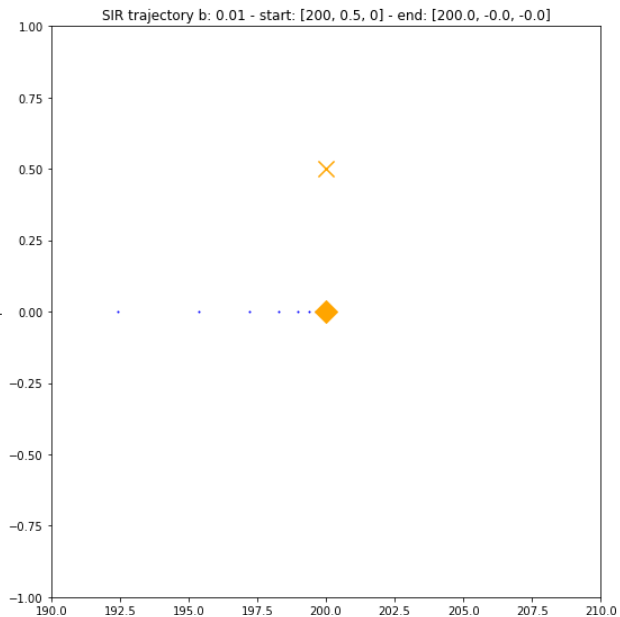
\includegraphics[width=0.3\textwidth]{images/task6_after_bif_1.png}}
    \hfill
    \subfloats[b]{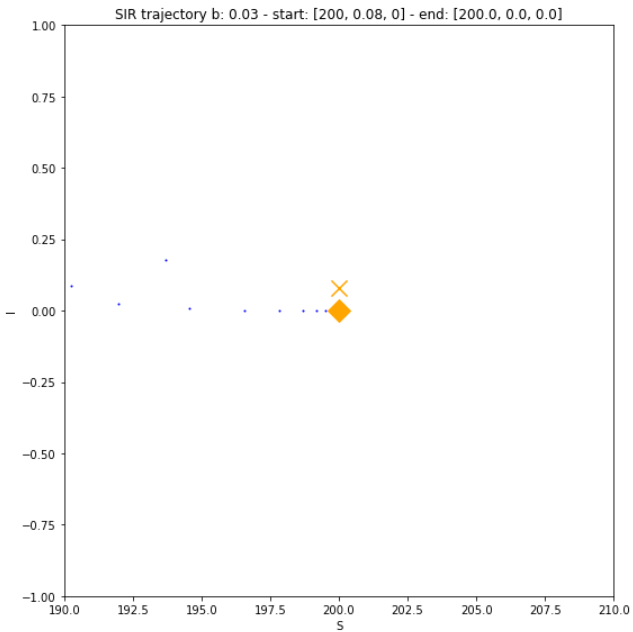
\includegraphics[width=0.3\textwidth]{images/task6_after_bif_2.png}}
    \hfill
    \subfloats[c]{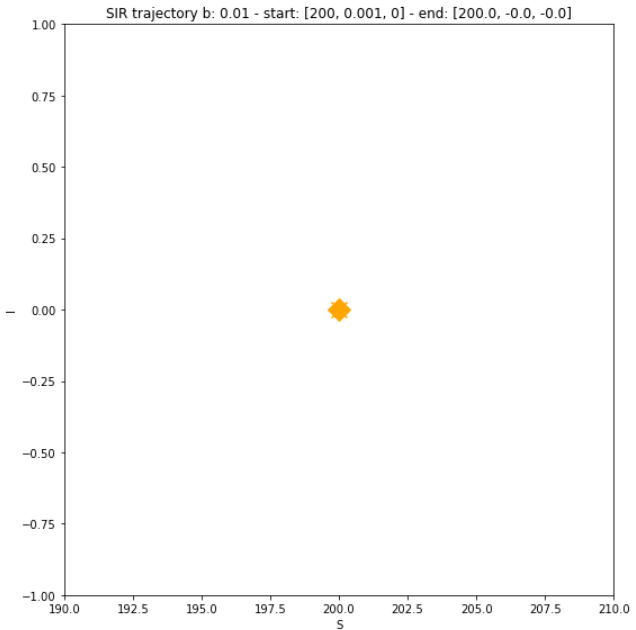
\includegraphics[width=0.3\textwidth]{images/task6_after_bif_3.png}}
    \vfill
    \subfloat[d]{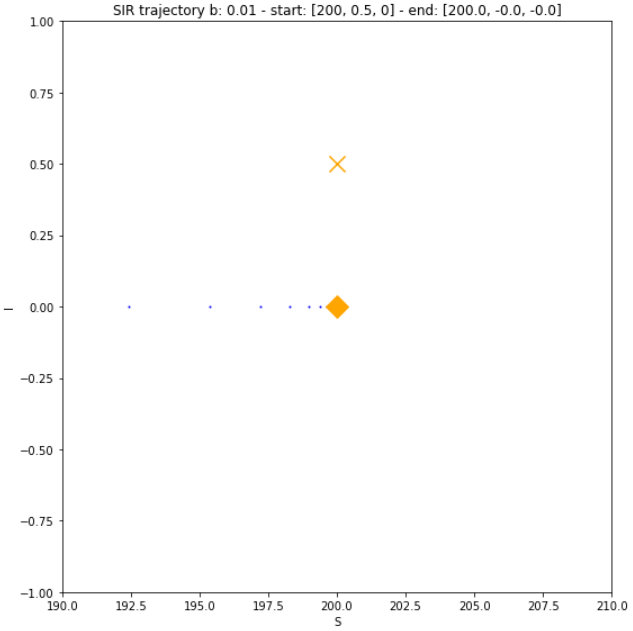
\includegraphics[width=0.3\textwidth]{images/task6_before_bif_1.png}}
    \hfill
    \subfloats[e]{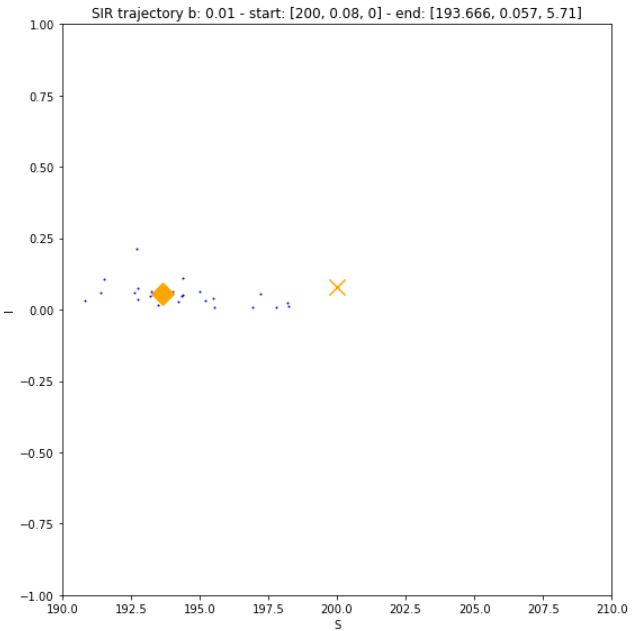
\includegraphics[width=0.3\textwidth]{images/task6_before_bif_2.png}}
    \hfill
    \subfloats[f]{\includegraphics[width=0.3\textwidth]{images/task6_before_bif_3.png}}
    \caption{With $b < 0.022$ the system always reaches $E_0=(\frac{A}{d}=200,\ 0,\ 0)$ ((a), (b), (c)).\\
    With $b > 0.022$:
    (d) starting far from $E_0$, the system reaches $E_0$ anyway;
    (f) starting near $E_0$, the system reaches $E_0$ anyway;
    (e) starting in between near and far from $E_0$, the system reaches the point [193.666, 0.057, 5.71).\\
    It is worth noticing that this point gets reached from many different starting points, even if in the figure only one example is shown for the sake of simplicity.}
    \label{fig:task5.6}
\end{figure}
\end{task}

\newpage
\bibliographystyle{plain}
\bibliography{Literature}

\end{document}